\section{Task: Import GPS Trail}
\label{sec:task_import_gps} 

This task allows importing of (D)GPS trails into the opened database, by parsing an NMEA file and writing the updates into the RefTraj DBObject.

\begin{figure}[H]
  \hspace*{-2.5cm}
    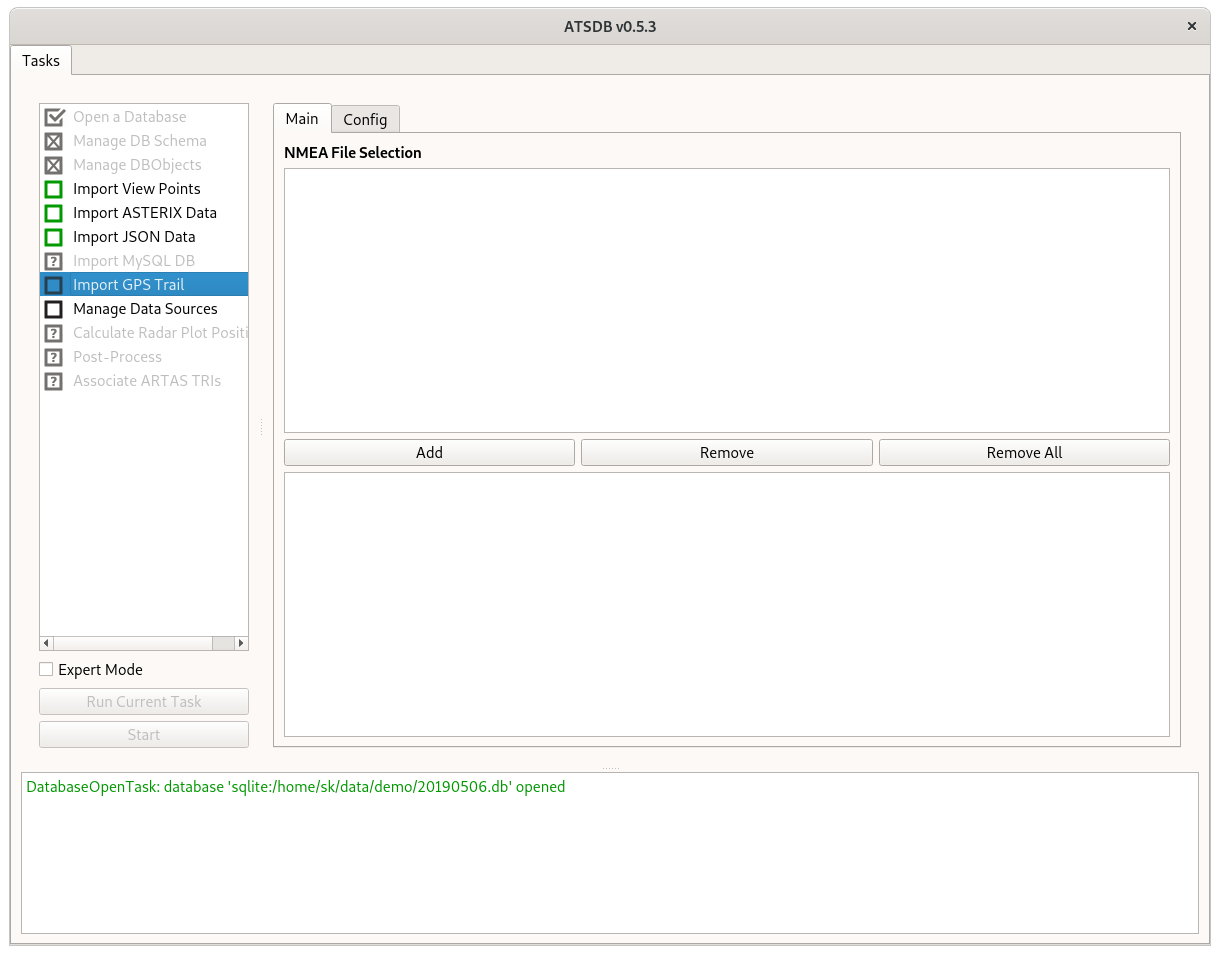
\includegraphics[width=19cm]{../screenshots/gps_import_task.png}
  \caption{Task: Import GPS Trail}
\end{figure}

There exist 4 tabs:

\begin{itemize}  
\item Main: File list and information text
\item Config: Configuration of data source and secondary information
\end{itemize}
\ \\

\subsection{Main Tab}

In the 'File Selection' list, a list of available NMEA files is given. Entries can be added using the 'Add' button or removed using either the 'Remove' or 'Remove All' buttons. \\

Below a text field is given which, after selection of an NMEA file, displays the content information and/or error messages. \\

\subsection{Config Tab}

\begin{figure}[H]
    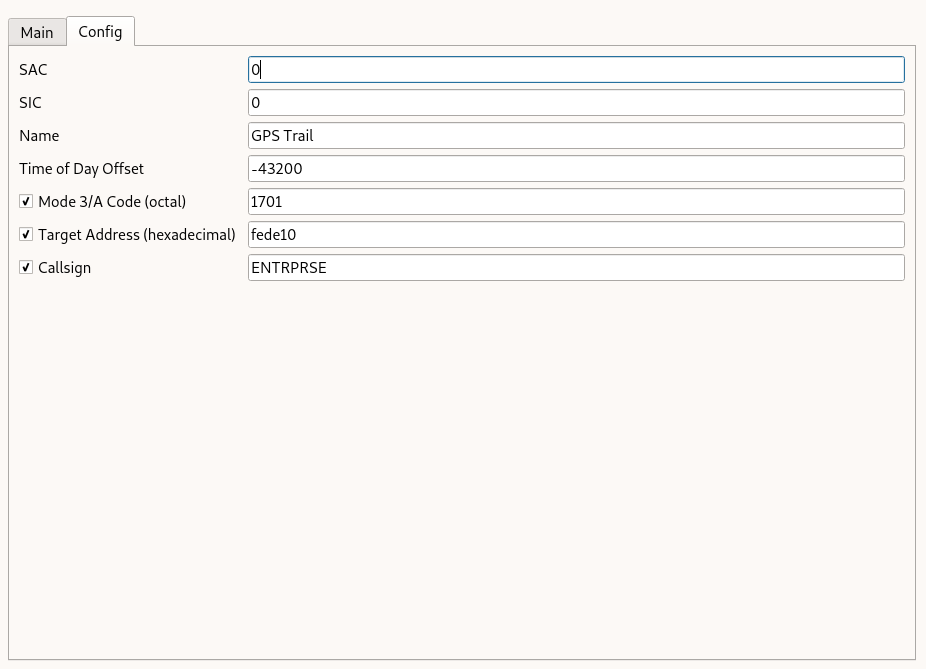
\includegraphics[width=16cm,frame]{../screenshots/gps_import_config.png}
  \caption{Task: Import GPS Trail Config}
\end{figure}

In the configuration tab, several configuration parameters can be set:

\begin{itemize}  
\item SAC: System area code of the reference data source
\item SIC: System identification code of the reference data source
\item Name: Name of the reference data source
\item Time of Day Offset: Time correction factor, in seconds. Set to 0 to disable.
\item Mode 3/A Code (octal): Mode 3/A code to be set. Uncheck checkbox to disable.
\item Target Address (hexadecimal): Mode S address to be set. Uncheck checkbox to disable.
\item Callsign: Target identification to be set. Uncheck checkbox to disable.
\end{itemize}
\ \\

\subsection{Running}

After selecting an NMEA file, using the 'Run Current Task' button the task can be performed.

\begin{figure}[H]
    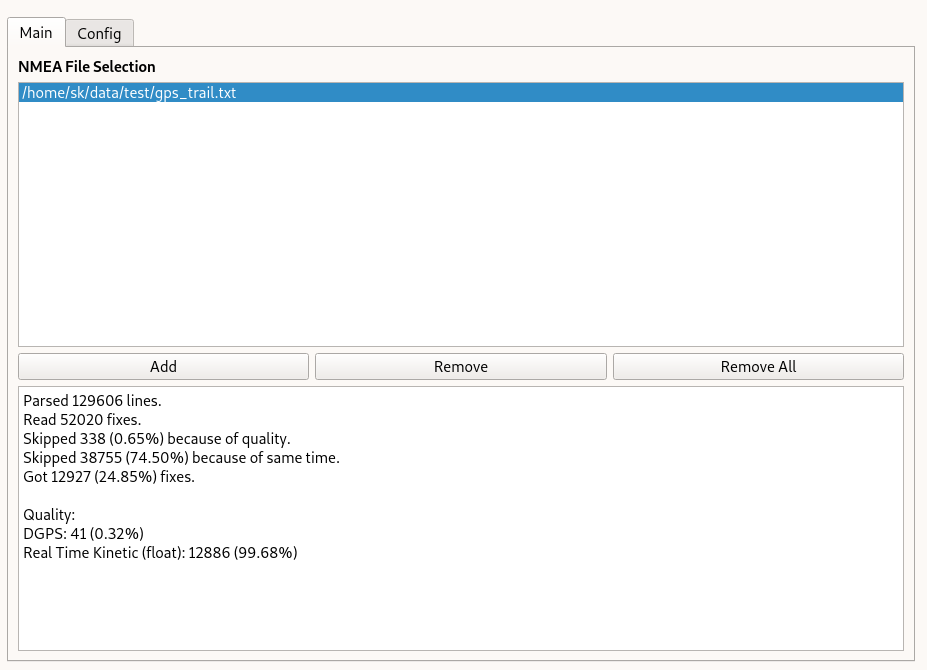
\includegraphics[width=16cm,frame]{../screenshots/gps_import_ready.png}
  \caption{Task: Import GPS Trail Ready}
\end{figure}
